\chapter[An approach to increase robustness in GNSS positionings]{\centering \begin{normalsize} \begin{Huge}
		An approach to increase robustness  in GNSS positioning
		\end{Huge} \end{normalsize}}
\label{ch:service_devel}

%\section{Workflow description}
%\section{GNSS raw: app for recording GNSS data from Android devices and sending them to a server}
%\section{Development of a low-cost permanent station for RTK positioning}

The GNSS positioning performances from smartphone devices is deeply exposed in chapter \ref{ch:quality_analisys}. The accuracy and precision obtainable in a relative post processing positioning are in the order of decimeters. Similar results can also be  obtained in real time, performing a RTK positioning. But, as highlighted by the tests performed, GNSS positioning from smartphones suffers from false fixed solutions, and outliers that compromise the robustness of the positioning itself. Those false fixed solution can be caused by many factors including the poor quality of the GNSS observables and the presence of external interferences such as multipath.
In this chapter, we present a solution to increase the robustness of GNSS RTK positioning using an Android device as a rover, and a low cost GNSS receiver as a base station. More in detail, in this chapter explains the architecture proposed highlighting the endpoints peculiarities and infrastructure realised from the communication between them. In the last part of the chapter particular attention is posed to the strategy implemented for increasing the robustness of the solution by means of the mitigation of the multipath error.
%
%\section{GNSS RTK positioning with Android devices}
The architecture of the GNSS RTK positioning procedure that we used to process GNSS data coming from Android smartphones consists of the following components:
\begin{itemize}
\item A smartphone for data acquisition;
\item A GNSS base station; 
\item A remote server for RTK processing.
\end{itemize}
The smartphone is supposed to be equipped with an Android App capable of reading GNSS raw observables, packing them in a proper way, and send them to a server running RTKLIB through a TCP socket. The base station must be capable of sending in real time it's observables together with it's precise coordinates to the server. The server is supposed to be capable of reading the input streams from the smartphone and from the base station, processing them with RTKLIB, and then returning the coordinates to the smartphone. 
The resulting architecture is shown in figure \ref{FIG:dev_rtk_arch}.
\begin{figure}[H] 
	\centering
	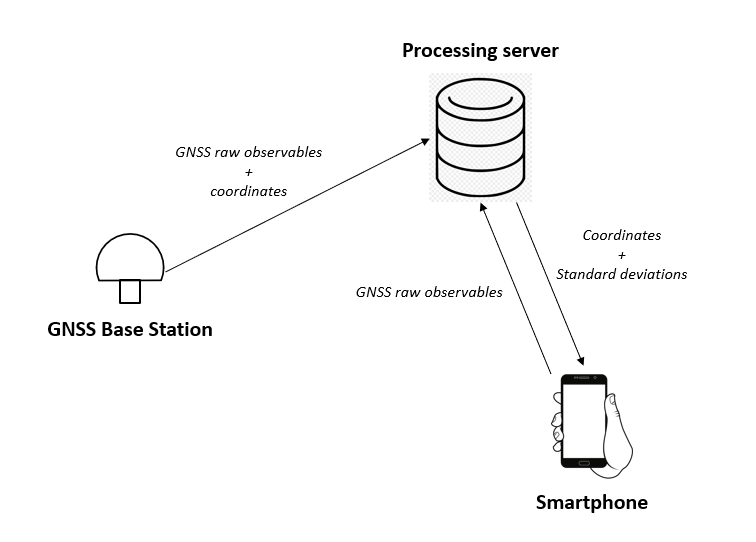
\includegraphics[scale=0.80]{fig/dev_rtk_arch.PNG} 
	\caption{Proposed architecture for robust RTK positioning with smartphone}
	\label{FIG:dev_rtk_arch} 
\end{figure}
The proposed system works with an ah-hoc GNSS base station assembled with a low cost GNSS receiver, but can be generalised by using an NRTK network instead. In the following sections the implementation of the different components are described in detail.
\section{GNSS base station}
\label{par:lige}
The first element of the developed architecture for GNSS RTK positioning with Android smartphones, is the GNSS base station. This paragraph describes the GNSS base station built, using a low cost hardware, and the software written for data acquisition and delivery. 
The hardware  is based on the dual frequency and multiconstellation GNSS receiver ublox ZED F9P. The performance of this receiver have been investigated in literature in many application \cite{Wielgocka:2021, Nguyen:2021,Hohensinn:2021}, and in open sky environment it can be considered a valuable alternative to geodetic-grade GNSS receivers \cite{janos:2021}. The GNSS receiver is coupled with the Hemisphere A45 antenna mounted in the rooftop of Gter's office, in Genoa. The base station hardware (see fig \ref{FIG:ligehw}) is completed with a Raspberry Pi used for data logging and delivery.
%
\begin{figure}[H] 
	\centering
	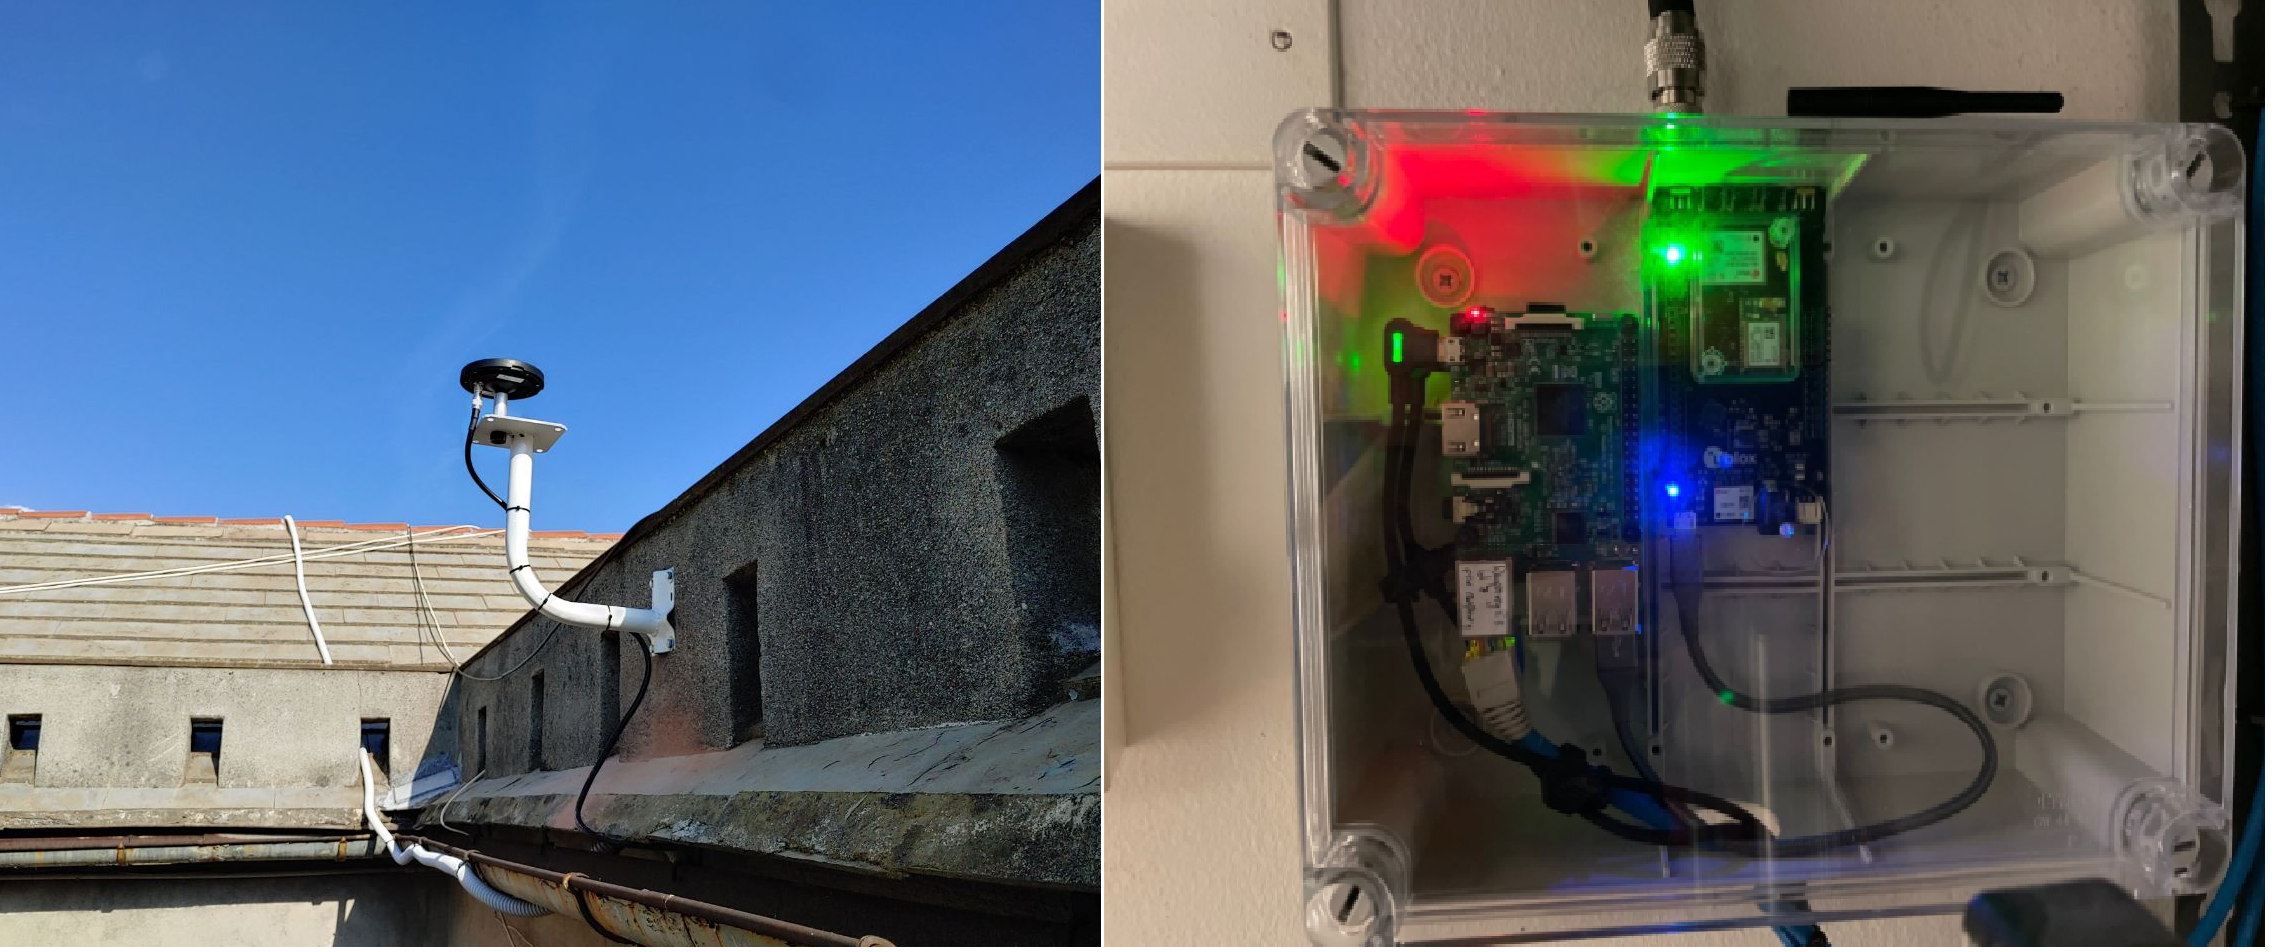
\includegraphics[scale=0.40]{fig/gnss_base_lige.png} 
	\caption{GNSS base station hardware}
	\label{FIG:ligehw} 
\end{figure}
%
The main functions of the GNSS station are:
\begin{itemize}
\item Publish the GNSS raw measurement stream  to users in real time over the Internet;
\item Recording hourly RINEX files and publish them on a ftp server.
\end{itemize}
%
In order to fulfil these two functions, the RTKLIB software was installed in the Raspberry Pi, and a few Python scripts were developed for background management of the processes. Figure \ref{FIG:ligesw} shows the developed software architecture.

\begin{figure}[H] 
	\centering
	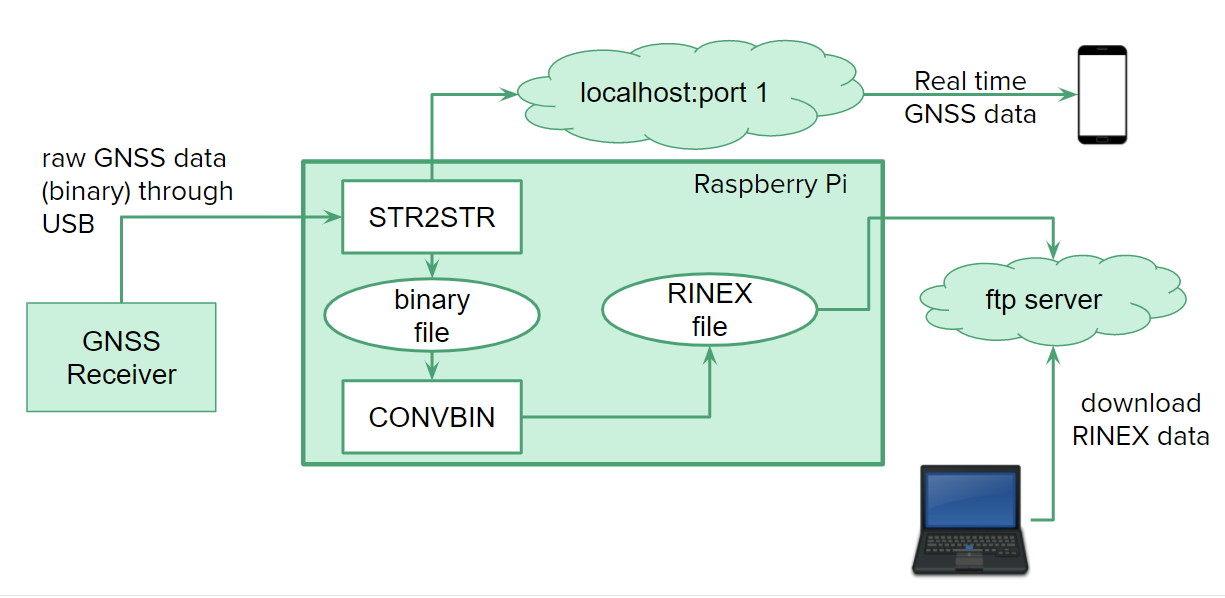
\includegraphics[scale=0.60]{fig/lige_sw_architecture.PNG} 
	\caption{GNSS base station software architecture}
	\label{FIG:ligesw} 
\end{figure}

In this GNSS base station the receiver is connected to the Raspberry Pi via USB, so the GNSS raw measurement observed by the receiver, must be transmitted to the Raspberry Pi through this channel.
By default the ublox GNSS receiver doesn't include the GNSS raw measurement in their stream coming out of the USB, but they have to be included manually. This operation can be done using the ublox management software u-center\footnote{\url{https://www.u-blox.com/en/product/u-center}}. Under the configuration menu, there's the possibility to include different messages to the output stream of the GNSS receiver. For having GNSS raw measurement in the USB output stream the messages to include are the ``RXM-RAWX", and the ``RXM-SRFBX". Once these messages are included, the GNSS receiver can properly work with RTKLIB modules. Another important option that can be set before using the GNSS receiver with RTKLIB is the acquisition rate. For this application the acquisition rate is set equal to 1Hz.

As shown in fig. \ref{FIG:ligesw}, the first block in the chain is the RTKLIB module STR2STR. This module is able to read an input stream and redirect it through different channels. In this case the input stream comes from the USB port, and it's redirected to a TCP port and to a file. The stream through the TCP port can be access by external user in order to perform a GNSS RTK positioning. The other output stream is saved to a file. This file is in binary format (ubx) so in order to be used for post processing application it shall be converted into RINEX format. This conversion can be done with the RTKLIB module CONVBIN. 
Process management is delegated to a couple of Python scripts: \textit{start\_acquisition} and \textit{stop\_and\_upload}. The first scripts simply launches an instance of STR2STR and saves in a temporary file the STR2STR's PID (Process ID), the path and the name of the local file created. When executed, the  \textit{stop\_and\_upload} script reads the information form the temporary file, kills the STR2STR and launches the CONVBIN software for RINEX conversion. Once the conversion is terminated, thanks to the Python's library \textit{ftplib} the RINEX file is upload to a ftp server and made available to users.
Properly inserted into \textit{"/etc/crontab"} file (i.e. the file that manages the automatic execution of software and scripts in a Raspberry Pi or more in general in a UNIX system) this two scripts allow having a continuous stream of GNSS raw observable through a TCP port and hourly RINEX file published in an FTP server. 
The code developed is also made available in the Gter's GitHub page\footnote{\url{https://github.com/gtergeomatica/GNSSBase_station_ublox}}.

\section{Android Application}
\label{sec:gnssraw}
%
The second component of the architecture  is a smartphone capable of accessing GNSS raw measurement. In order to make the smartphone working in this architecture, a specific Android App, named  ``GNSS Raw", is conceived and developed. The purpose of this app is to read data from the Android device in which it is installed, sending them to a remote server, and reading and plotting the position computed by the server with those data.
The application is written in Java and it is compatible with all devices running an Android version higher than 7.0 Nougat. During the PhD work we have developed two versions of the App. More specifically, in the second release we have improved data preparation and added services to visualise the computed position, run the app in background, and disable duty cycle directly in the app (for Full Track surveys) without the need to disable it from the developer options menu. This last feature is available only for devices having Android version higher than 12 (API level 31).

The application, based on the GNSS Logger app released by Google\footnote{\url{https://github.com/google/gps-measurement-tools/tree/master/GNSSLogger}} is composed by 5 different menu:
\begin{itemize}
\item Measurement
\item Plot
\item Map
\item Files
\item Settings
\end{itemize}
In the rest of the section we will describe each functionality while focusing on important points in 
the implementation of the Java code.
%
\subsubsection*{Measurement}
The Measurement menu presents a very simple GUI (Graphical User Interface) as shown in figure \ref{FIG:gnssraw_measurement}, and is used to to start and stop data recording.
\begin{figure}[H] 
	\centering
	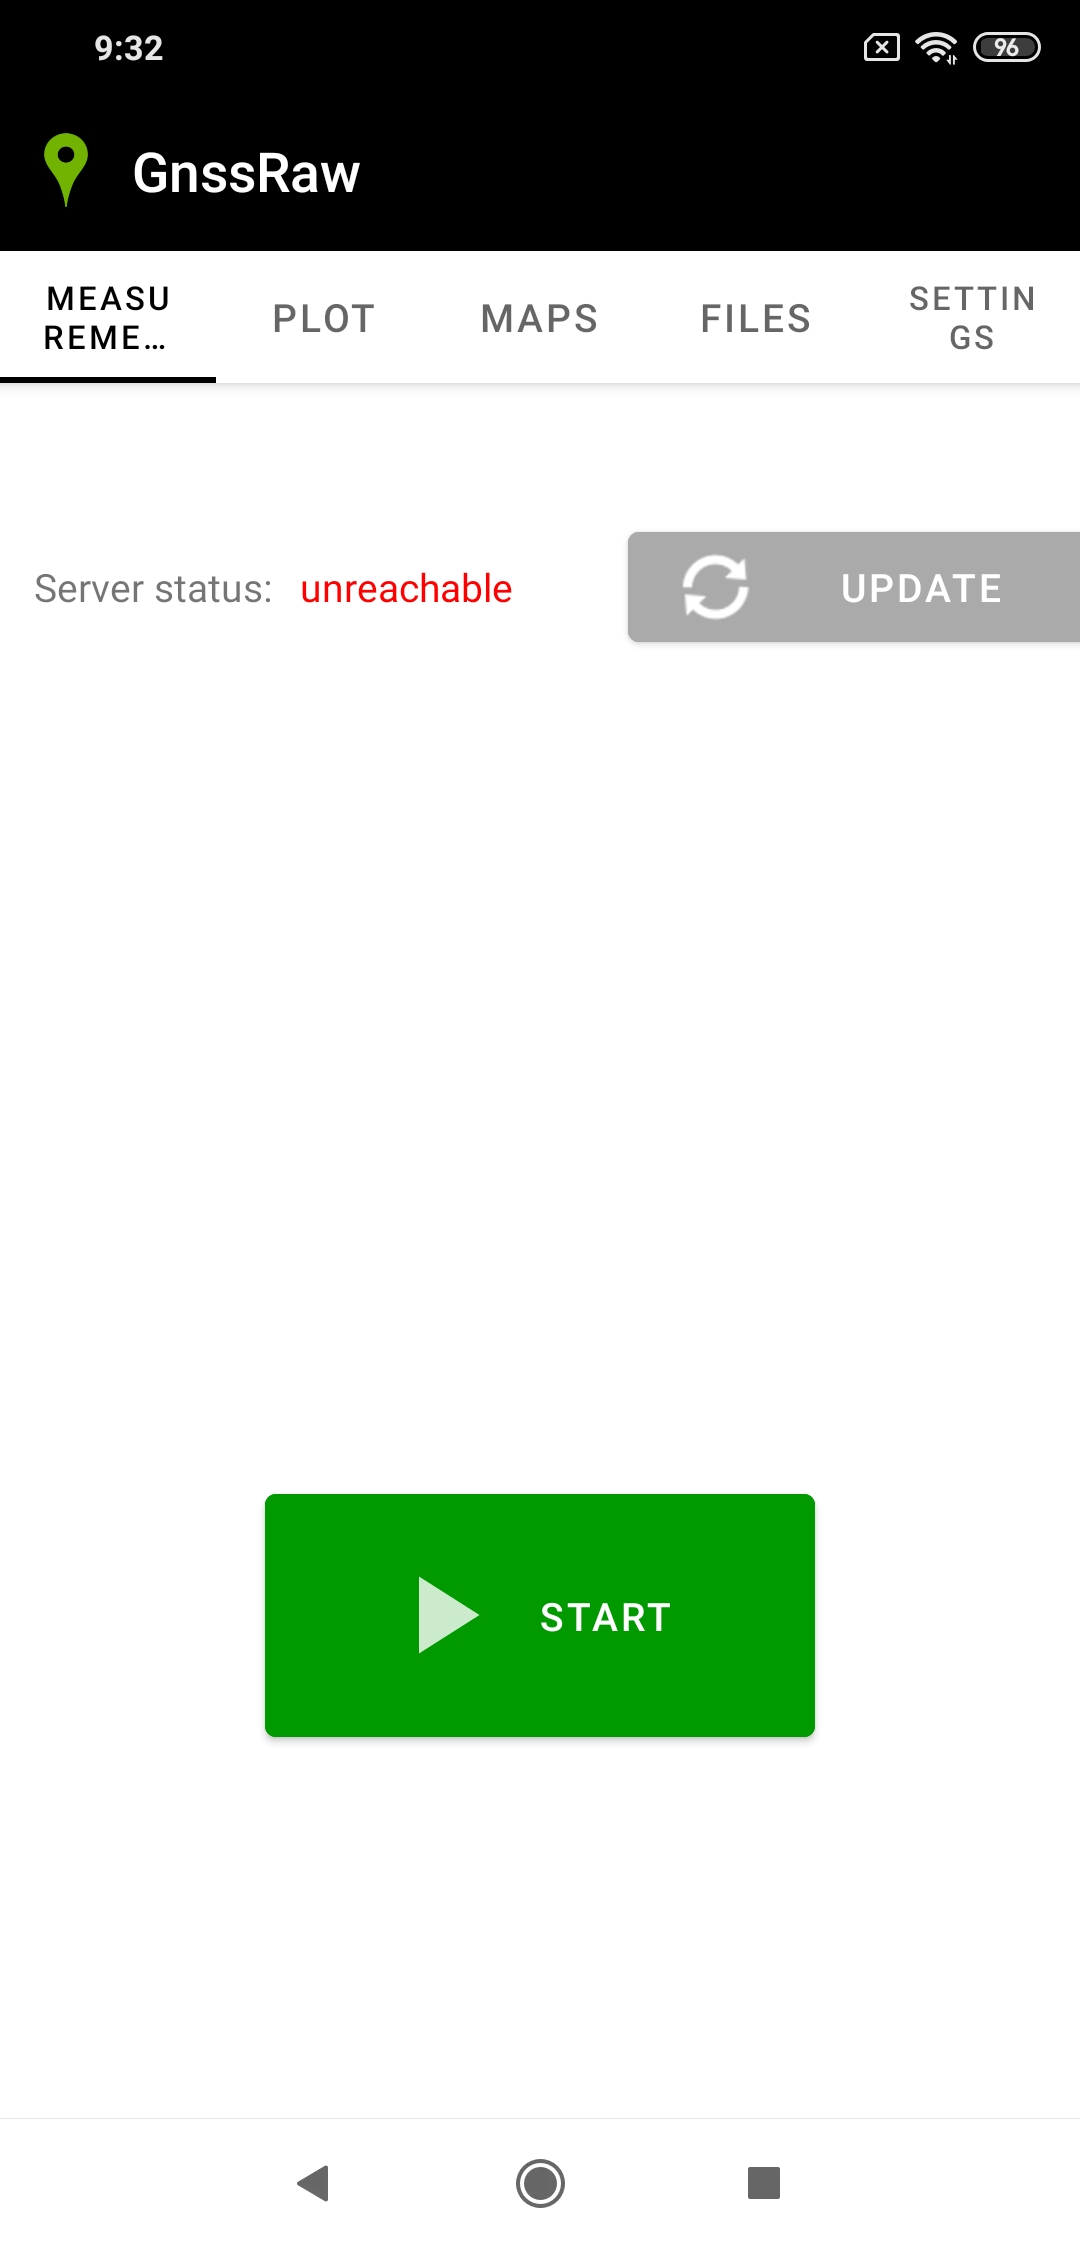
\includegraphics[scale=0.15,frame]{fig/gnssraw_measurement.jpg} 
	\caption{GNSS Raw: Measurement menu}
	\label{FIG:gnssraw_measurement} 
\end{figure}
When the start button is pushed, the GNSS raw measurement data (see chapter \ref{ch:SoA}) are saved in a local file and sent to a remote server (when reachable) in real time. 
The procedure for accessing the GNSS raw data from the smartphone GPS receiver are described next.
\subsubsection*{Data Acquisition}
The Java code that implements data acquisition, processing and communication is listed in Appendix \ref{appendix:androidcode}
organized in accord with the class diagram depicted in Fig. \ref{FIG:class_diagram}. 
\begin{figure}[H] 
	\centering
	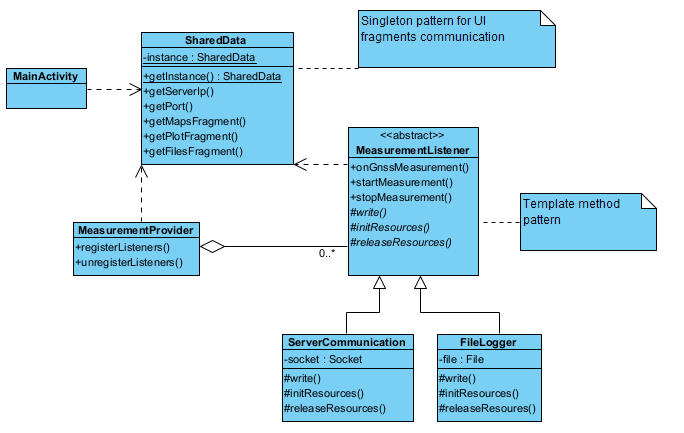
\includegraphics[scale=0.80,frame]{fig/class.png} 
	\caption{Class diagram}
	\label{FIG:class_diagram} 
\end{figure}
More specifically, we defined the following Java classes:
\begin{itemize}
\item 
the class \verb+MeasurementProvider+ that contains the software configuration of the GNSS engine (e.g. managers, listeneres, and sampling intervals);
\item 
the class  \verb+MeasurementListener+ that specifies the  data collection listeners;
\item 
the class \verb+ServerCommunication+ (that extends 
\verb+MeasurementListener+) that provides the API communication layer between the smartphone and the RTKLIB server.
\item 
the singleton class \verb+SharedData+ is used to encapsulate all data used in the application, to share data among different tabs, 
and to decouple the application logic from its view component (the fragments used in the UI).
\end{itemize}
The \verb+MeasurementProvider+ class creates a \verb+LocationManager+ object and the callbacks and parameters used for setting up the GNSS data acquisition.  
The \verb+LocationManager+ class provides access to the system location services, and in particular allows applications to obtain periodic updates of the device's geographical location. Starting from API level 24, using this class it's also possible to access GNSS raw measurements. In order to get those data a specific callback has been created.\footnotemark{A callback is a function  that is passed into another function as an argument and is expected to execute after some specific type of event.} The callback is invoked every time  a new measurement occurs and it is used for receiving GNSS satellite data. Each measurement contains raw and computed data identifying a satellite. 
The sampling rates are defined via the static attributes \verb+LOCATION_RATE_GPS_MS+ (1 second) 
and \verb+LOCATION_RATE_NETWORK_MS+ (1 minute).

The public method \verb+onGnssMeasurementsReceived+, used in the above mentioned class, reports the latest collected  GNSS measurements from the GNSS engine via  listener.
The listener provides a callback to be invoked when the \verb+MeasurementManager+ updates the sensors and signals data. 
The callback invokes the  method \verb+onGnssMeasurementsReceived+ of the \verb+MeasurementListener+ class. The method invocation received  \verb+event+ object that contains the raw measurement data in the format of the Android GNSS raw data library.
To correctly process those measurements, it's necessary to send to the RTKLIB server all the measurements referred to the same epoch in an unique block. For this reason, the implemented callback checks the epoch of every measurement and creates an unique string with all the measurement referred to the same epoch. This string is sent to the server in order to be processed.

More specifically, the method \verb+onGnssMeasurementsReceived+ computes the current timestamp using the \verb+getClock()+ method of the corresponding event. Every satellite measurement shares the same clock value up to milliseconds. The milliseconds timestamp of each single piece of data can be extracted from the event object via the \verb+event.getMeasurements()+ method. 
Data of the different satellites are then packaged into a single string delimited by two special sentinels ("NB" and "FB") via 
by invoking  the method \verb+getMeasurementInfo+.
The packaging phase is executed in the body of the listener 
(not on separate threads) since it does not seem to affect the performance of the app.   
%
\subsubsection*{Data Transmission}
%
In order to set up the Client-Server communication simple TCP sockets from the standard Java network library (java.net) were used.
To correctly set up the communication with the server, the server's IP and the port, must be specified in the relatives boxes (figure \ref{FIG:gnssraw_settings}. The reachability status of the server can be checked by the user in the "Measurement" menu.
The communication is active by default, but the application gives also the possibility to turn it off. In this case the application doesn't perform any positioning, but simply records GNSS raw data. 
Assuming the server is reachable, the app sends the packaged GNSS raw measurements to the server using the \verb+write+ method of the  \verb+ServerCommunication+ class.
Differently from the data preparation phase, 
the \verb+ServerCommunication+ class employs a thread pool in order to schedule data transmission on a dedicated thread to avoid to block the UI in case of transmission delays.
%
\subsubsection*{Plot}
The Plot menu (figure \ref{FIG:gnssraw_plot}) is activated only when the start button is pushed. Similarly to the Google GNSS logger app, this menu, shows the $SNR$ trend over time. This parameter is a good indicator of the quality of the incoming signal, and it's useful to keep it monitored during a survey in order to understand which satellites may cause problems in the positioning. The GNSS Raw app allows to filter this graph by constellation or by individual satellite.

\begin{figure}[H] 
	\centering
	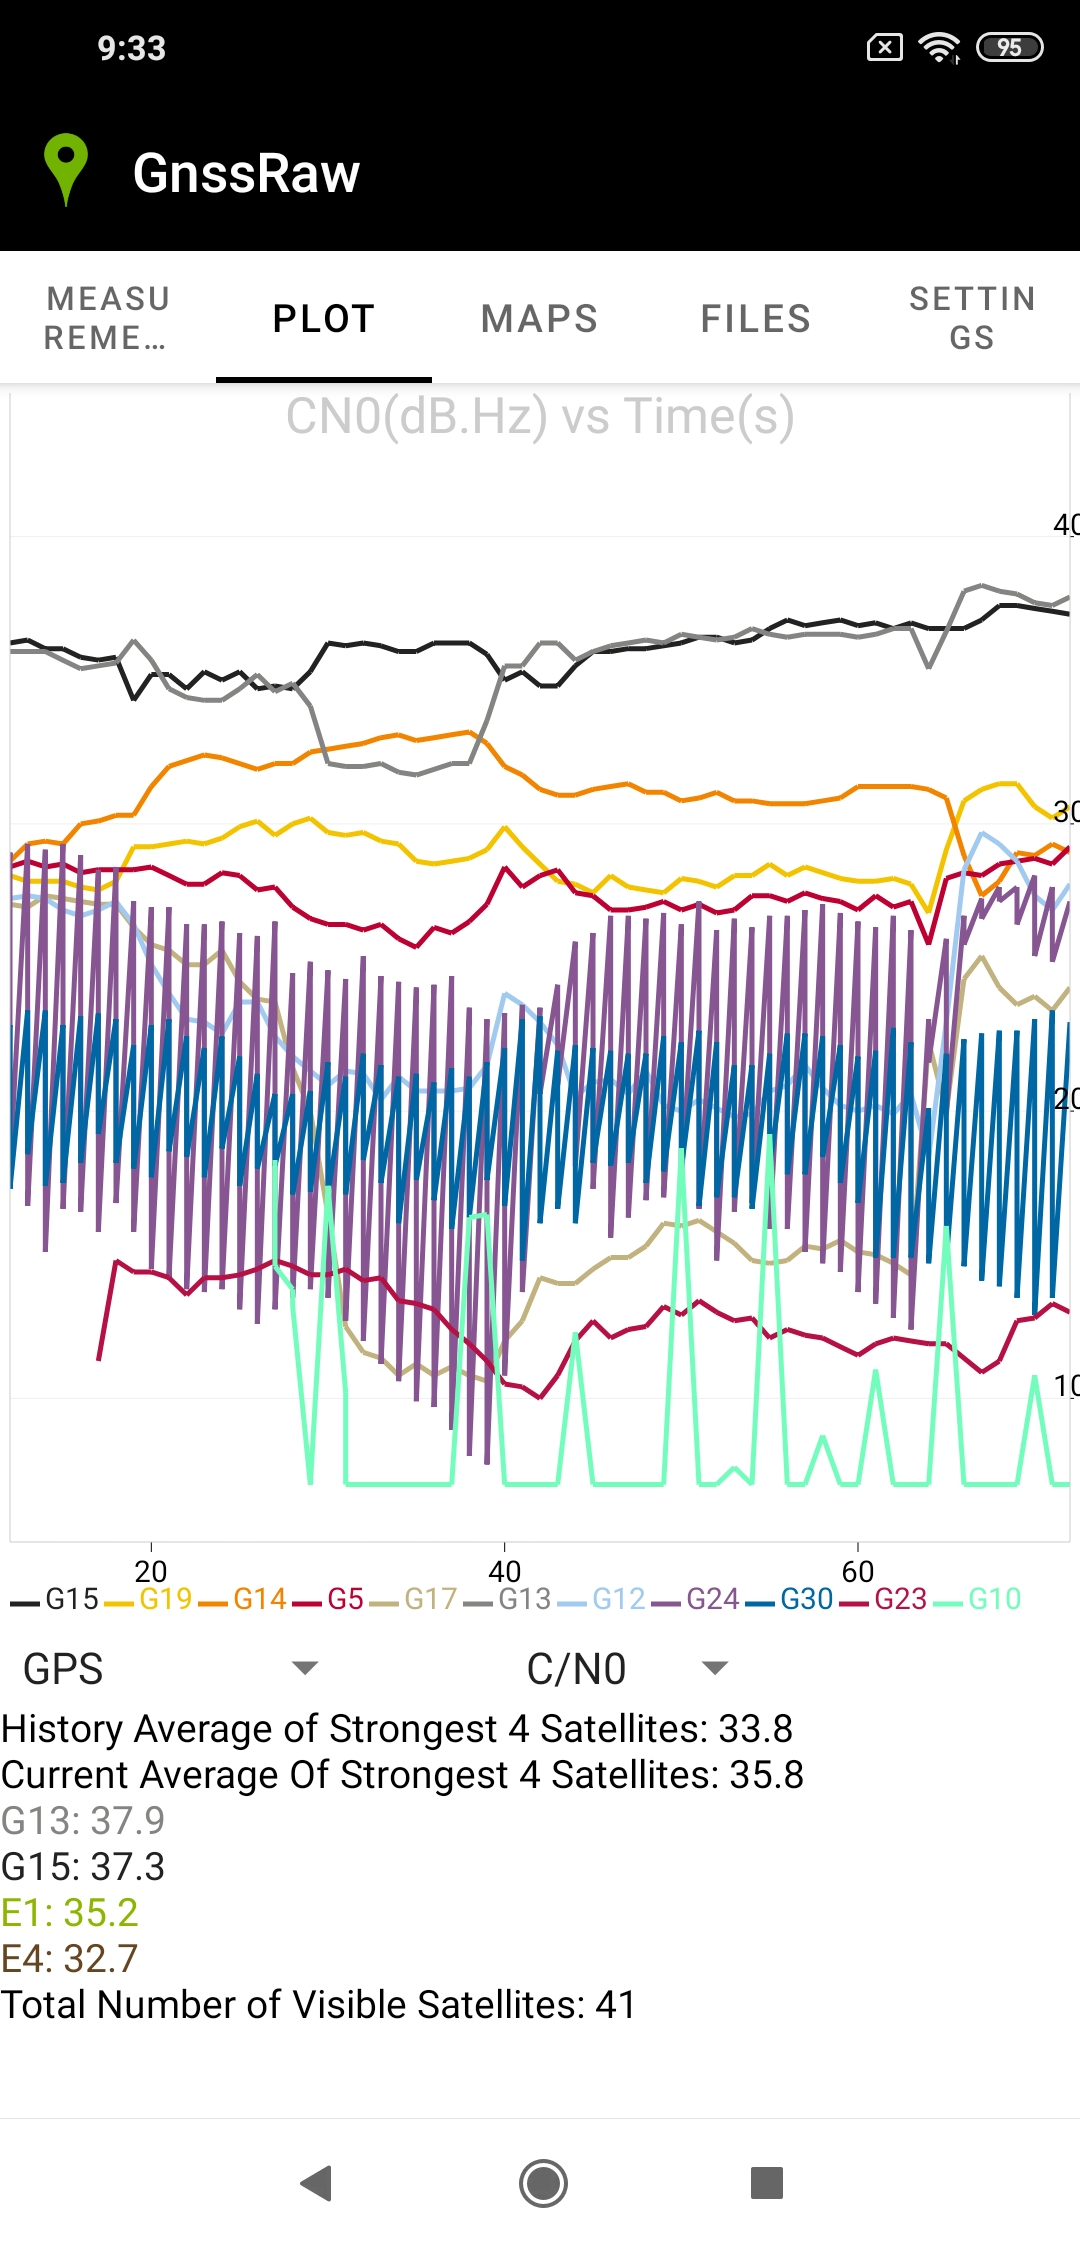
\includegraphics[scale=0.15,frame]{fig/gnssraw_plots.jpg} 
	\caption{GNSS Raw: Plot menu}
	\label{FIG:gnssraw_plot} 
\end{figure}

The GNSS raw, implements a menu for viewing the recorded files with GNSS raw measurement (figure \ref{FIG:gnssraw_file}), without using the smartphone's integrated file manager. In order to keep order between all the recorded files, the filename criteria adopts the simple rules ``GNSS\_Log" suffix followed by the date. This menu also allows user to share the recorded data through common sharing channels, and gives the possibility to eliminate them from the local storage memory. 

\begin{figure}[H] 
	\centering
	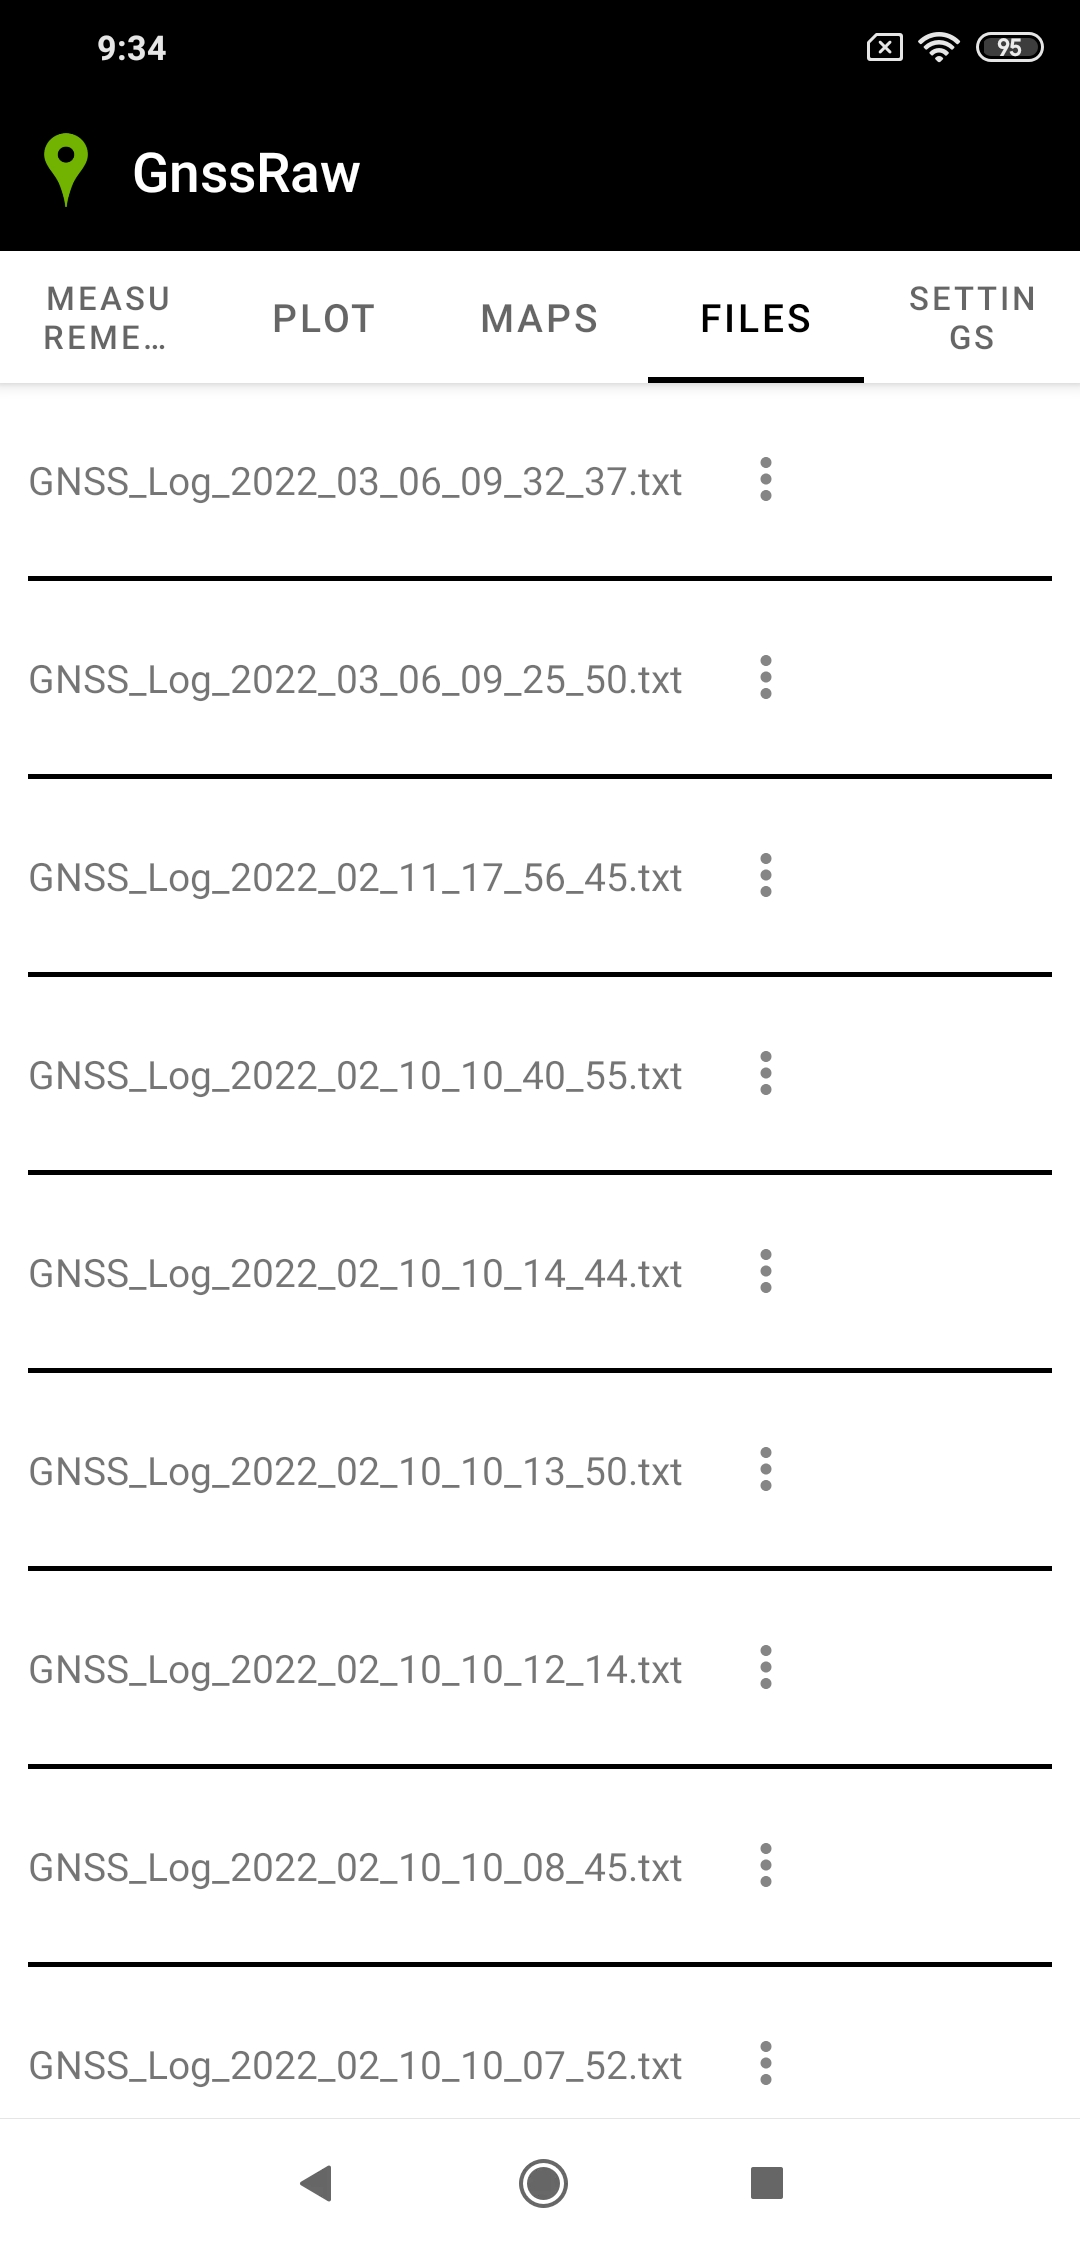
\includegraphics[scale=0.15,frame]{fig/gnssraw_files.jpg} 
	\caption{GNSS Raw: File menu}
	\label{FIG:gnssraw_file} 
\end{figure}
\subsection*{Settings}
The Settings menu (figure \ref{FIG:gnssraw_settings}) is mainly used to set up the communication between the smartphone and the remote server running RTKLIB.

\begin{figure}[H] 
	\centering
	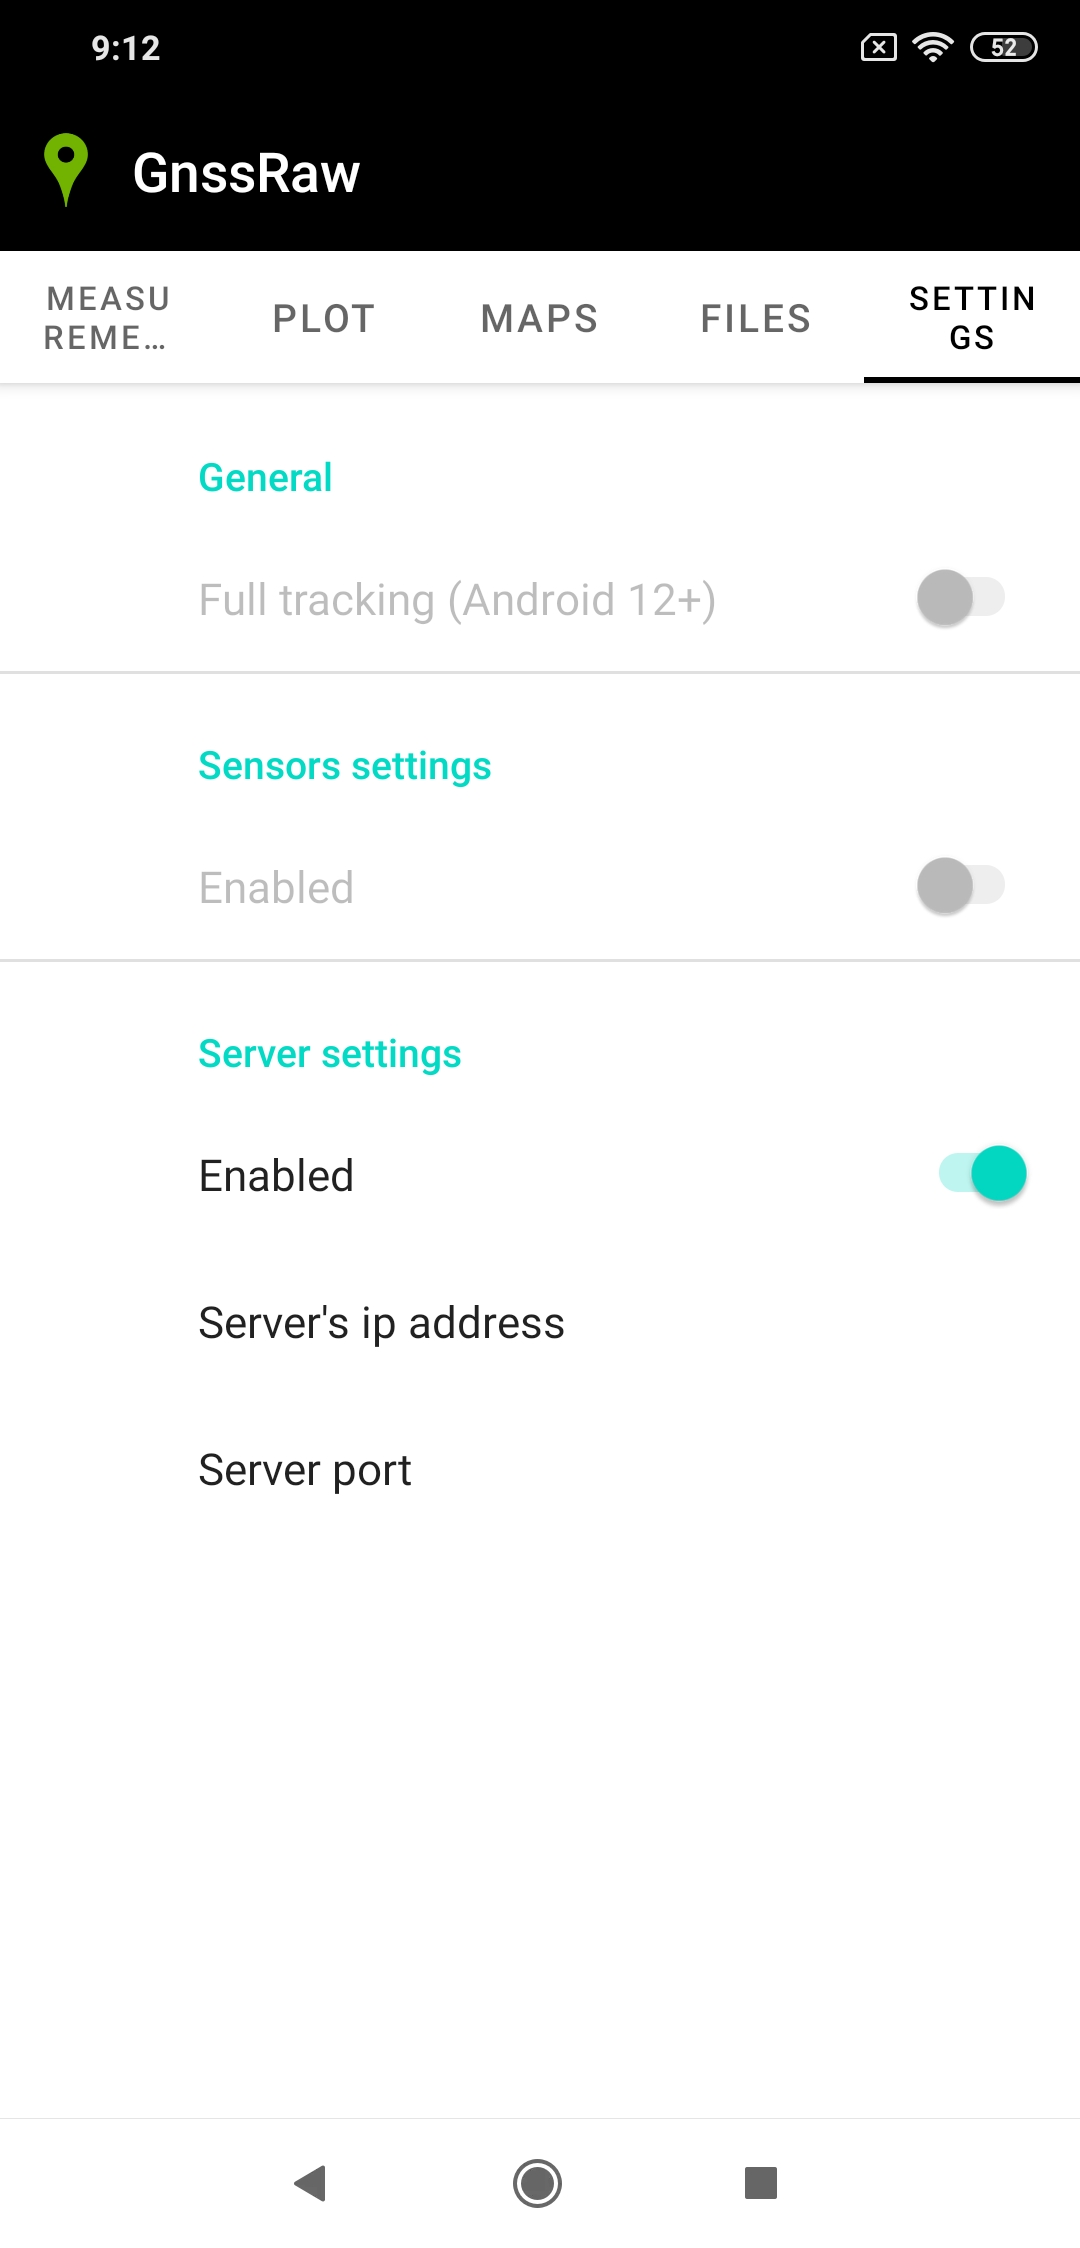
\includegraphics[scale=0.15,frame]{fig/gnssraw_settings.jpg} 
	\caption{GNSS Raw: Settings menu}
	\label{FIG:gnssraw_settings} 
\end{figure}
\subsection*{Map}
 The results of the processing (i.e. the coordinates and the associated standard deviations) are sent to a tcp server on the same host, by means of a native RTKLIB function. The GNSS raw app connects to this server using another socket and get the processed data. Those data are than parsed and plotted in the Map menu (figure \ref{FIG:gnssraw_map}).   
The marker in the map changes color accordingly to the solution status. In particular the marker becomes green if the solution is Fix, yellow is the solution is Float and red if the solution is Stand Alone (i.e. the relative positioning couldn't be performed).

\begin{figure}[H] 
	\centering
	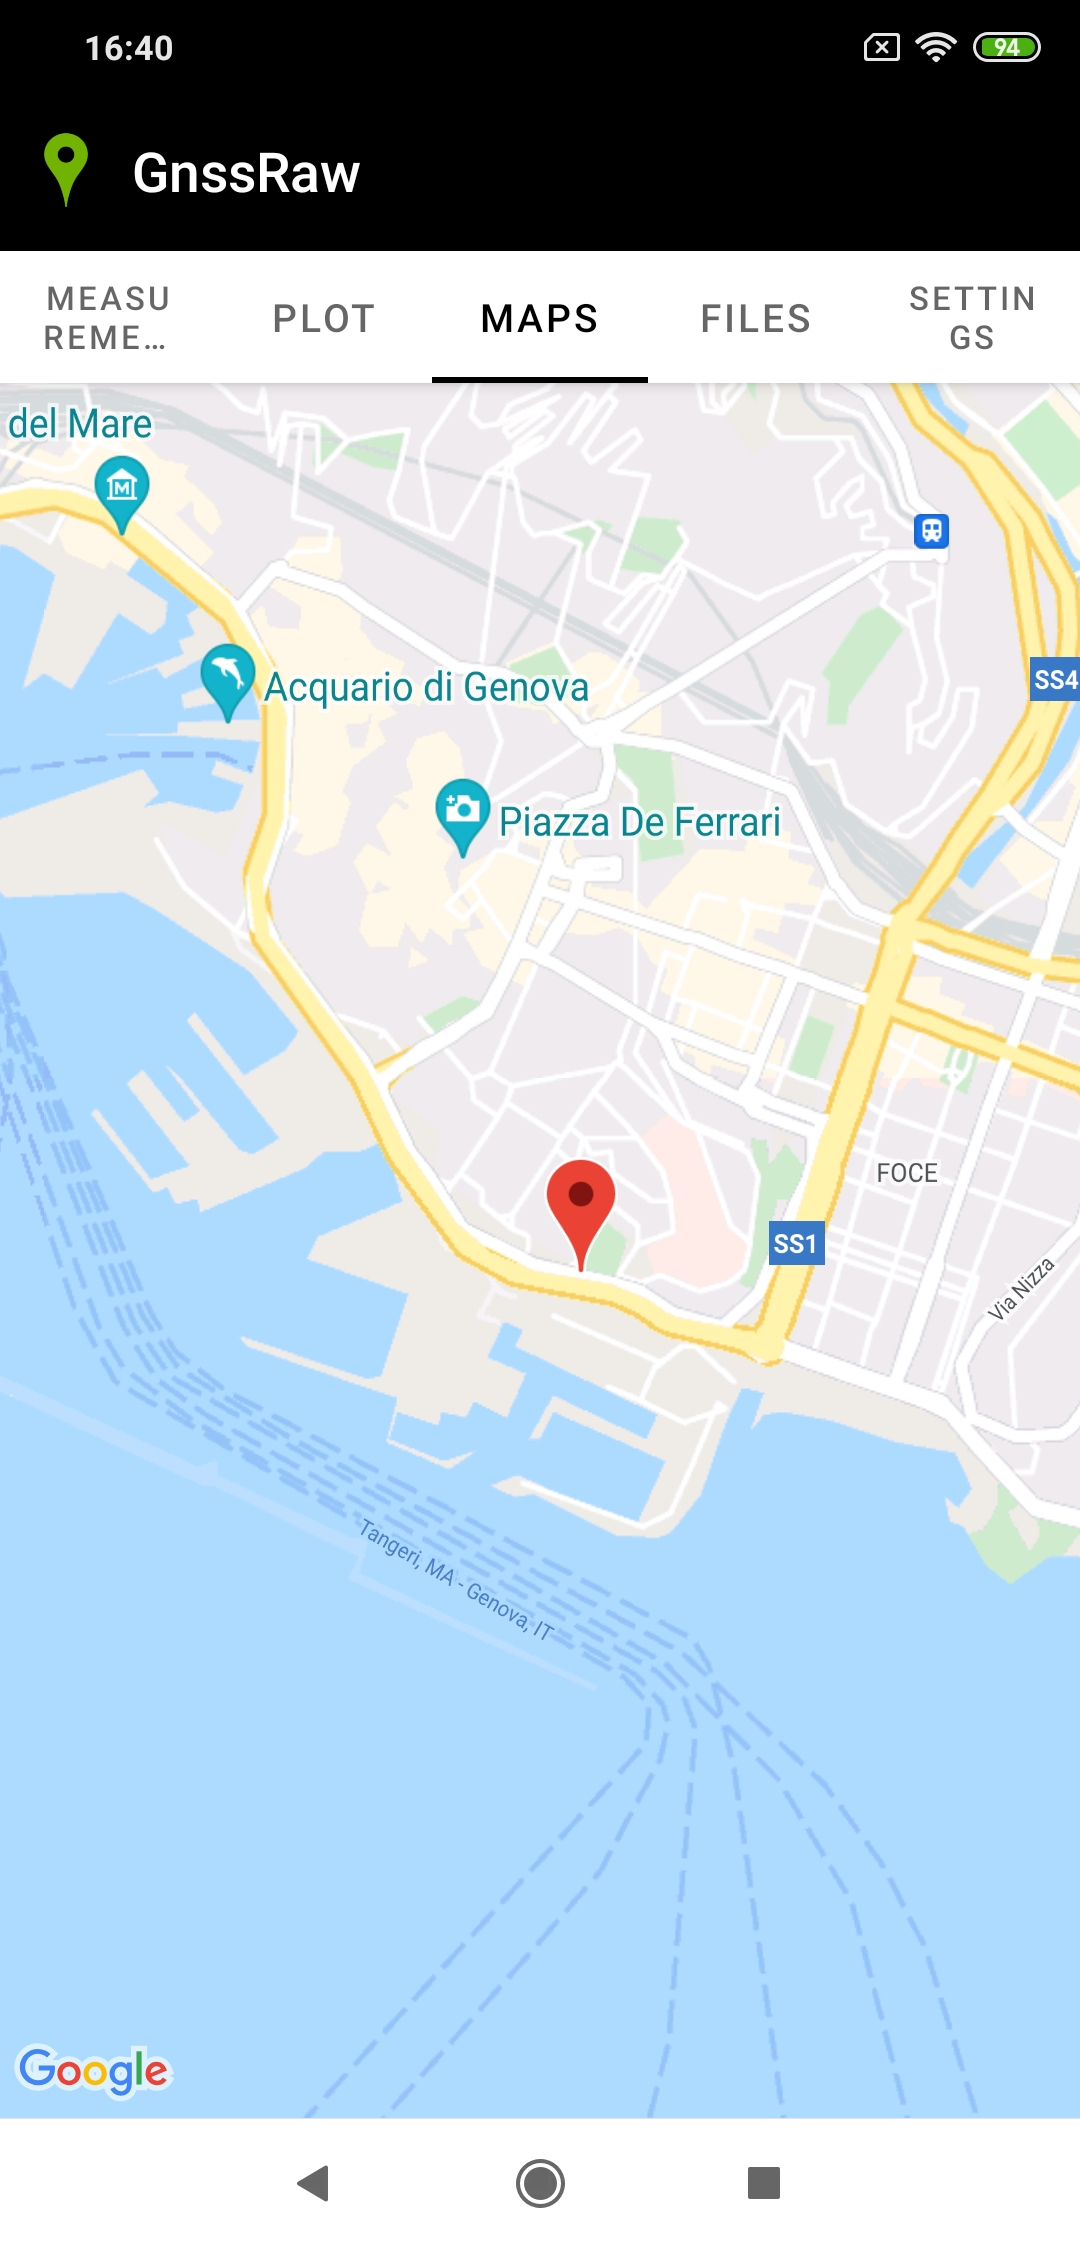
\includegraphics[scale=0.15,frame]{fig/gnssraw_maps.jpg} 
	\caption{GNSS Raw: Map menu}
	\label{FIG:gnssraw_map} 
\end{figure}
The source code of the app has been also translated and optimized to Kotlin language, which is now supported by Google as an official language for Android apps. The Kotlin code of the app is available on a branch of the GitHub repository of the app. \\
The GNSS raw application has been designed in order to read and send to the server not only GNSS raw data, but also data coming from the other sensor embedded in the smartphone. The main idea is to send to the server, also data coming from accelerometer, gyroscope and magnetometer, to investigate the possibility to perform server side, an integration between GNSS and INS data from smartphone. This kind of integration is not object of this work and the function to record data from other sensor in the smartphone is still under development.
%
\section{RTKLIB Server}
\label{sec:modified_rtklib}
The last component of the architecture is a remote server for GNSS positioning. The server should have installed an RTKLIB version for data processing and should be able to communicate in real time with both the smartphone and the Base station though tcp sockets. In the specific case an Ubuntu 20.04 server has been chosen. Concerning the GNSS processing, the standard version of RTKLIB only few formats for input GNSS data, including the standard ones (RTCM 3, RTCM2 and BINEX) and some GNSS manufacturers proper binary format. The original version of RTKLIB is not capable of working in real time with GNSS data coming from Android devices, as the format in which they are accessed is not recognised by the software. The ``Android format" is the one generated by the ``GNSS raw" app (see par \ref{sec:gnssraw}). In order to overcome this issue, in the ambit of this work, the original version of RTKLIB was modified, in order to perform, a RTK GNSS positioning using data coming from an Android smartphone.  This section explains in details the software modification done to make RTKLIB compatible with Android format. In rtksvr.c there's the \textit{decoderaw} function used to decode input data and saving them in the proper structure to be elaborated. The \textit{decoderaw} function has 3 different cases depending on input data format, and for each cases implements the following function:
\begin{itemize}
\item \textit{input\_rtcm2} for decoding RTCM v.2 data
\item \textit{input\_rtcm3} for decoding RTCM v.3 data
\item \textit{input\_raw} for decoding binary data from the supported receivers
\end{itemize}

Differently from \textit{input\_rtcm2} and \textit{input\_rtcm3} functions, the \textit{input\_raw} requires as an argument, in addition to the data to be decoded, the format of that data. This parameter must be specified by the user in the configuration file. For every supported format RTKLIB implements a different decoding function. The main RTKLIB modification consists in the generation of a new format together with it's relative decoding function, called \textit{decode\_gterAndroid} used to decode the data sent from the ``GNSS raw" app (see par. \ref{sec:gnssraw}). Before entering this function, an entire block of data must be recognised from the input stream. This operation allows to pass to the \textit{decode\_gterAndroid} function a set of observables all referring to the same epoch, which is essential for the rest of the processing. Data recognition is based on the fact that each block of data referred to the same epoch, is packed in a specific way, and has an identification character needed for its synchronisation. After a block of data is recognized the \textit{decode\_gterAndroid} function is executed.
The first operation performed by the function is to recognise and isolate within the block of data read the subsets of observables corresponding to each single satellite. Then, for each set of observables, using the strategies described in chapter \ref{ch:SoA}, the following parameters are calculated:
\begin{itemize}
\item Satellite ID
\item Frequency and observation code
\item GPS week and GPS second of week
\item Pseudorange
\item Carrier phase 
\item Doppler
\item Signal to Noise Ratio
\end{itemize}
Once they have been computed, the quantities are saved in the proper RTKLIB structure in order to be used in the part of the software workflow. In the pseudo-range and carrier phase computation some controls are implemented as suggested in \cite{GSA_wp:2016}. In particular for the pseudo-range computation it is necessary to control the decoding status of the Time Of Week (TOW) value, an essential parameter for the correct generation of pseudo-range. 
In other words even a small uncertainty on the TOW could lead to a completely wrong value of the pseudo-range which in turn could significantly degrade the quality of the final positioning. The decoding status of the TOW can be retrieved using the GNSS Android API. By comparing this value with some defined constants (see table \ref{tab:api_constants}), it is possible to distinguish whether the TOW is properly decoded or not. In case the TOW results not properly decoded the pseudo-range it is not computed.

Concerning the carrier phase generation, a check is made on the validity status of the observable. In this case the GNSS 
Android API presents a specific field, called \textit{AccumulatedDeltaRangeState}, used for this purpose. Furthermore this field is also used to verify the presence of cycle slips. Considering the high noisiness of GNSS observables from smartphones a second check is implemented on carrier phase generation. This second check is performed using the field \textit{AccumulatedDeltaRangeUncertaintyMeters} that provides and estimation of the uncertainty in meters on the accumulated delta range quantity. In the modified RTKLIB version a new configuration parameter, called \textit{maxadru} was introduced, to discard all the carrier phase measurements whose \textit{AccumulatedDeltaRangeUncertaintyMeters} parameter is higher than the specified value. By default the \textit{maxadru} parameter is equal to 0.1 meters.
%
\section{Multipath Mitigation Heuristics}
One of the major external interference that degrade GNSS 
positioning is multipath. The effect of this interference is well described by its name: a satellite-emitted signal arrives at the
receiver from different directions (i.e following different paths). Multipath effect is mainly caused by reflecting surfaces
nearby the receiver. For this reason, it frequently happens  in urban canyons, a typical scenario in which smartphone are used.
Multipath effect may also occur when using low cost GNSS receivers equipped with low quality antennas, such as the smartphone's ones. For this reason a good strategy to improve the robustness in GNSS positioning from Android devices should aim at mitigating the multipath error. 

Multipath mitigation can be performed at the Antenna, Receiver (Signal Processing) and Navigation Solution Level \cite{Bhuiyan:2010}. 

%Concerning antenna level mitigation possible solutions are 

In this work the multipath mitigation is attacked at software level, using an algorithm, called MDP (Multipath Detection Parameter) conceived by Gter. In the following section the algorithm is explained in detail together with its implementation in RTKLIB.
\subsection{The MDP Algorithm}
The MDP algorithm consists in two main parts: the first one concerning multipath detection, and the second one concerning multipath mitigation.
The multipath detection part is based on the SNR (Signal to Noise Ration) value and a new variable called MDP (Multipath Detection Parameter). The aim of the MDP value is to create a variable representative for multipath effect for single frequency GNSS receivers, starting from the observation equation. 
The observation equations for GNSS are:
\begin{equation}
    \begin{matrix}
        P(t_{1})=\rho(t_{1})+\Delta T_{r}^{s}(t_{1}) + Ion(t_{1}) + Trop(t_{1}) + Mult(t_{1}) + \epsilon \\
        L(t_{1})=\rho(t_{1})+\Delta T_{r}^{s}(t_{1}) - Ion(t_{1}) + Trop(t_{1}) + mult(t_{1}) + \lambda N+ \epsilon
    \end{matrix}
\label{eq:obs_multipath}
\end{equation}
where
\begin{itemize}
\item \textit{P(t\textsubscript{1})} is the pseudorange observable at instant \textit{t\textsubscript{1}}
\item \textit{L(t\textsubscript{1})} is the carrier phase observable at instant \textit{t\textsubscript{1}}
\item $\rho(t_{1})$ is the geometric range between the satellite and the receiver at instant \textit{t\textsubscript{1}}
\item $\Delta T_{r}^{s}(t_{1})$ is the global time unknown at instant \textit{t\textsubscript{1}}
\item $Ion(t_{1})$ is the ionospheric effect on the signal at instant \textit{t\textsubscript{1}}
\item $Trop(t_{1})$ is the tropospheric effect on the signal at instant \textit{t\textsubscript{1}}
\item $\lambda N$ is the phase ambiguity
\item $Mult(t_{1})$ is the code multipath
\item $mult(t_{1})$ is the phase multipath
\item $\epsilon$ represents residual errors due to noise.
\end{itemize}

The reported equations are valid for GPS and Galileo. If GLONASS constellation is considered, then the inter-channel bias should also be added to the model.

One common approach to isolate the multipath effect from equations \ref{eq:obs_multipath} is to compute their difference \cite{Bisnath:2001}. The result is the so-called sentinel variable:
\begin{equation}
    S(t_{1}) = P(t_{1})-L(t_{1}) = 2Ion(t_{1})- \lambda N + (Mult(t_{1}) - mult(t_{1}))
\label{eq_sentinel}
\end{equation}
The definition of MDP variable requires two assumptions. 
Considering a sufficiently high acquisition rate (i.e. 1 Hz), we can 
assume that:
\begin{itemize}
    \item The ionosphere effect is equal between 2 consecutive epochs;
    \item The phase ambiguity is equal between 2 consecutive epochs.
\end{itemize}
Based on these assumptions, the MDP variable is defined as:
\begin{equation}
    MDP=S(t_{2})-S(t_{1})=\{ [Mult(t_{2})-mult(t_{2})]-[Mult(t_{1})-mult(t_{1})]\}+\epsilon
\label{eq:mdpvariable}
\end{equation}
Hence, as shown in equation \ref{eq:mdpvariable}, the MDP variable is representative of the effect of multipath effect and   
residual errors due to noise.
\subsubsection{MDP: Detection Algorithm}
The detection algorithm compares the SNR and  MDP parameters to
static and dynamic threshold values as explained below.
\paragraph*{SNR Threshold} The multipath detection part proposed in the MDP algorithm exploits also the SNR value, which is not a specific indicator for multipath but for noise in general. The aim of checking also the SNR mask is to identify outliers which can be caused by multipath, other external interference, or can refer to corrupted data.
More specifically, for the SNR parameter 
a static threshold is set before running the positioning procedure. The value to be assigned to the SNR threshold depends on several factors, such as the quality of the GNSS antenna and the environmental conditions of the survey. The optimal value to assign to the threshold is still object of research. In this work, it is determined experimentally by trying different configurations, as explained in the chapter \ref{ch:mdp_results}.
Epoch by epoch for each acquired observable the SNR value is compared to the chosen threshold: if the SNR value is lower than the threshold, the observable is flagged with a so-called SNR flag.
\paragraph*{MDP Threshold}
The MDP is a parameter specifically designed to identify data affected by multipath. Under normal conditions, i.e. absence of multipath, the variable MDP is expected to have a white noise trend, and it's values depend on the entity of residual errors due to noise. In case of incoming multipath, the MDP variable is expected to have some outliers. The aim of the MDP threshold than is to identify those outliers, as they indicate multipath affected data. Two difference MDP thresholds were introduced in this work: a static one and a dynamic one. The static MDP threshold is used in a similar way to the SNR threshold. The optimal MDP threshold value is still object of research and in this work, it is determined experimentally by trying different configurations, as discussed in the chapter \ref{ch:mdp_results}.  Once the MDP static threshold is set, epoch by epoch for each acquired observable the MDP value is computed and compared to the threshold. The observable is then flagged with a so-called MDP flag if:
\begin{equation}
|MDP| \geq mdpthreshold 
\label{eq:mdpthres}
\end{equation}
Concerning the MDP, also an adaptive threshold was proposed. This adaptive threshold is computed considering a statistical analysis on previous epochs. 
The heuristics is based on an additional parameter, $N$, that defined the length of the observation window (number of epochs to be analysed). As the aim of the MDP threshold is to detect outliers, the Chebyshev's inequality is used for its definition. In fact, Chebyshev’s inequality states that, considering a broad range of probability distributions, 88.89\% of values lies within three standard deviations of the mean \cite{chebyshev:1}. The MDP adaptive threshold is then defined as:
\begin{equation}
mdpthreshold = \mu \pm 3\sigma
\label{eq:mdpthres_din}
\end{equation}
where
\begin{itemize}
    \item $\mu$ is the mean MDP value on $N$ previous epochs;
    \item $\sigma$ is the standard deviation of the $N$ previous MDP values;
\end{itemize}
In this case the observable is flagged if:
\begin{equation}
MDP \leq \mu -3\sigma \vee MDP \geq \mu + 3\sigma
\label{eq:mdpthres_dyn}
\end{equation}
\paragraph*{Initialization Phase}
The detection part of the algorithm when the MDP dynamic threshold is chosen, needs an initialization time equal to $N$ times the acquisition rate. Therefore, for example, if the acquisition rate is 1Hz and $N$ is equal to 60, the detection algorithm needs 1 minute to reach a complete operating status. 
\paragraph*{Detection Phase}
Based on the current values of the MDP and SNR flags, the detection algorithm implements 3 different criteria to state if the observable is affected by multipath. Those criteria are:
\begin{itemize}
    \item Crit 1.: Only MDP flag
    \item Crit 2.: MDP flag and SNR flag
    \item Crit 3.: MDP flag or SNR flag
\end{itemize}
Figure \ref{FIG:mdp_workflow} summarises the resulting detection algorithm.
\begin{figure}[H] 
	\centering
	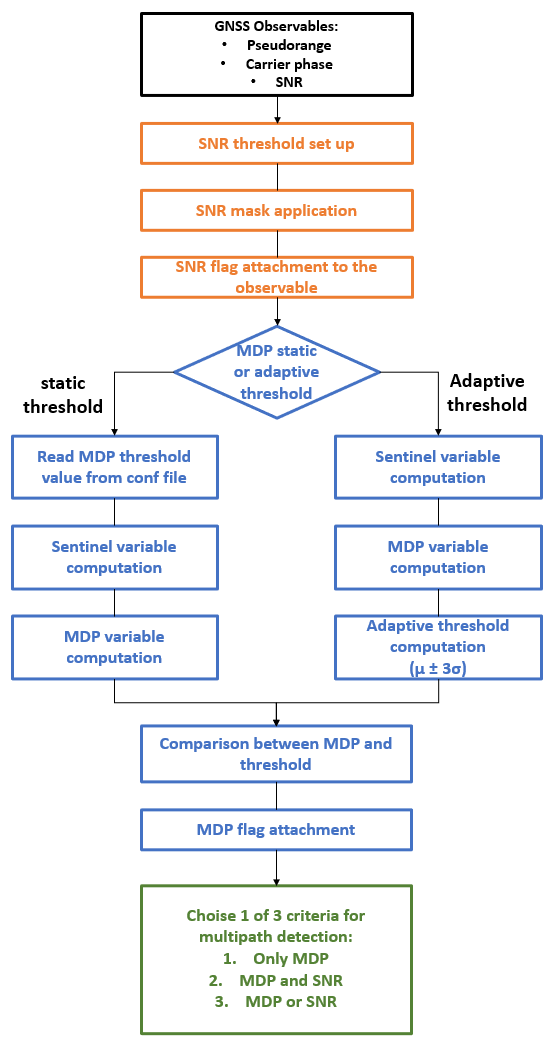
\includegraphics[scale=1]{fig/mdpscheme.png} 
	\caption{MDP: Detection part of the algorithm}
	\label{FIG:mdp_workflow} 
\end{figure}
\clearpage
For each epoch, using this procedure, a set of observables potentially affected by multipath is identified. 
The detection phase is used then to trigger the mitigation procedure.
\subsubsection{MDP: Mitigation Algorithm}
The aim of the mitigation algorithm is to retrieve a more accurate and precise GNSS positioning taking into account multipath-affected observables. One possible way to mitigate multipath effect is to exclude the multipath affected observables. This heuristics runs into the risk of excluding too many GNSS observables, hence producing a poor quality result due to missing redundancies in the 
observables. In order to avoid this scenario, a good way to proceed is to consider associated different weights to the multipath-affected GNSS observables. 

Since the MDP is integrated in RTKLIB, the new proposed weight to be associated with the multipath affected observables is based on the weight that the software associates with the observables.
As previously described RTKLIB uses a weight matrix defined as:
\begin{equation}
\textbf{W}=diag\left(\sigma_{1}^{-2}, \sigma_{2}^{-2}, ...,\sigma_{n}^{-2}\right)
\label{eq:rtklib_weight_matrix}
\end{equation}
In eq. \ref{eq:rtklib_weight_matrix}, $\sigma_{n}^{2}$ is the variance associated to the n\textsuperscript{th} observable defined as:
\begin{equation}
\sigma_{meas}^{2}=F^{s}R_{r}\left(a_{\sigma}^{2}+\frac{b_{\sigma}^{2}}{sinEL_{r}^{s}}\right)
\label{eq:rtklib_weight_matrix1}
\end{equation}
where:
\begin{itemize}
    \item $F^{s}$ is the satellite system error factor which is equal to 1 for GPS, Galileo, QZSS and BeiDou, equal to 1.5 for BEIDOU and equal to 3 for GLONASS
    \item $R_{r}$ is the code/carrier‐phase error ratio
    \item $a_{\sigma}, b_{\sigma}$ are the carrier‐phase error factor a and b in meters
\end{itemize}
    
Furthermore the software adds to this variance other contributions, so the final equation becomes:

\begin{equation}
\sigma_{obs}^2= \sigma_{meas}^2+\sigma_{eph}^{2}+\sigma_{ion}^{2}+\sigma_{trop}^{2}+\sigma_{bias}^{2}
\label{eq:rtklib_variance_matrix1}
\end{equation}

where
\begin{itemize}
    \item $\sigma_{eph}$ is the standard deviation of ephemeris and clock error in meters
    \item $\sigma_{ion}$ is the standard deviation of ionosphere correction model error in meters
    \item $\sigma_{trop}$ is the standard deviation of troposphere correction model error in meters
    \item $\sigma_{bias}$ is the standard deviation of code bias error in meters [m]
\end{itemize}


In order to take into account of the multipath effect, the variance of the observables identified as potentially affected by multipath, is incremented adding a new component. This component, is based on the sigma-$\epsilon$ model \cite{Brunner:1999,Wieser:2000} used to weight GNSS observables by means of their SNR value. A new term has been added to this model in order to take into account also the multipath effect by means of the MDP value. The resulting term, called \textit{mdp variance}, is expressed by:

\begin{equation}
\sigma_{mdp}^{2}= mdp^{2}+C\cdot 10^{-\frac{SNR}{10}}
\label{eq:rtklib_mdp_variance}
\end{equation}

Where $C$ is a model parameter equal to 0.244 m\textsuperscript{2}DB-Hz for L1 frequency.
The proposed weight model is defined in a such way to amplify the impact of the multipath effect (MDP variable) with respect to external noise (SNR). 
 Since the weight associated to the observables is equal to the inverse of its variance (see eq. \ref{eq:rtklib_weight_matrix}), the weight of the observable decrease as its MDP value increase. Furthermore using the proposed MDP variance, the multipath affected observable are weighted in a different way depending on their MDP values: observables affected by a large multipath error (high MDP value) will have a lower weight with respect to observables having a lower multipath error (i.e. lower MDP value). Furthermore the MDP variance takes into account also the SNR value. As the SNR value decreases (i.e. the observable noise increases), the MDP variance associated to the variable increases and consequently its weight decreases.
%l'approccio proposto verrà validato sperimentalmente

An experimental validation of the proposed algorithm will be presented in the next chapter.
%nel prossimo capitolo verrà presentata una validazione sperimentale dell'algoritmo proposto... 
